% Options for packages loaded elsewhere
\PassOptionsToPackage{unicode}{hyperref}
\PassOptionsToPackage{hyphens}{url}
\PassOptionsToPackage{dvipsnames,svgnames,x11names}{xcolor}
%
\documentclass[
  letterpaper,
  number,
  review,
  3p]{elsarticle}

\usepackage{amsmath,amssymb}
\usepackage{iftex}
\ifPDFTeX
  \usepackage[T1]{fontenc}
  \usepackage[utf8]{inputenc}
  \usepackage{textcomp} % provide euro and other symbols
\else % if luatex or xetex
  \usepackage{unicode-math}
  \defaultfontfeatures{Scale=MatchLowercase}
  \defaultfontfeatures[\rmfamily]{Ligatures=TeX,Scale=1}
\fi
\usepackage{lmodern}
\ifPDFTeX\else  
    % xetex/luatex font selection
\fi
% Use upquote if available, for straight quotes in verbatim environments
\IfFileExists{upquote.sty}{\usepackage{upquote}}{}
\IfFileExists{microtype.sty}{% use microtype if available
  \usepackage[]{microtype}
  \UseMicrotypeSet[protrusion]{basicmath} % disable protrusion for tt fonts
}{}
\makeatletter
\@ifundefined{KOMAClassName}{% if non-KOMA class
  \IfFileExists{parskip.sty}{%
    \usepackage{parskip}
  }{% else
    \setlength{\parindent}{0pt}
    \setlength{\parskip}{6pt plus 2pt minus 1pt}}
}{% if KOMA class
  \KOMAoptions{parskip=half}}
\makeatother
\usepackage{xcolor}
\setlength{\emergencystretch}{3em} % prevent overfull lines
\setcounter{secnumdepth}{5}
% Make \paragraph and \subparagraph free-standing
\ifx\paragraph\undefined\else
  \let\oldparagraph\paragraph
  \renewcommand{\paragraph}[1]{\oldparagraph{#1}\mbox{}}
\fi
\ifx\subparagraph\undefined\else
  \let\oldsubparagraph\subparagraph
  \renewcommand{\subparagraph}[1]{\oldsubparagraph{#1}\mbox{}}
\fi


\providecommand{\tightlist}{%
  \setlength{\itemsep}{0pt}\setlength{\parskip}{0pt}}\usepackage{longtable,booktabs,array}
\usepackage{calc} % for calculating minipage widths
% Correct order of tables after \paragraph or \subparagraph
\usepackage{etoolbox}
\makeatletter
\patchcmd\longtable{\par}{\if@noskipsec\mbox{}\fi\par}{}{}
\makeatother
% Allow footnotes in longtable head/foot
\IfFileExists{footnotehyper.sty}{\usepackage{footnotehyper}}{\usepackage{footnote}}
\makesavenoteenv{longtable}
\usepackage{graphicx}
\makeatletter
\def\maxwidth{\ifdim\Gin@nat@width>\linewidth\linewidth\else\Gin@nat@width\fi}
\def\maxheight{\ifdim\Gin@nat@height>\textheight\textheight\else\Gin@nat@height\fi}
\makeatother
% Scale images if necessary, so that they will not overflow the page
% margins by default, and it is still possible to overwrite the defaults
% using explicit options in \includegraphics[width, height, ...]{}
\setkeys{Gin}{width=\maxwidth,height=\maxheight,keepaspectratio}
% Set default figure placement to htbp
\makeatletter
\def\fps@figure{htbp}
\makeatother
% definitions for citeproc citations
\NewDocumentCommand\citeproctext{}{}
\NewDocumentCommand\citeproc{mm}{%
  \begingroup\def\citeproctext{#2}\cite{#1}\endgroup}
\makeatletter
 % allow citations to break across lines
 \let\@cite@ofmt\@firstofone
 % avoid brackets around text for \cite:
 \def\@biblabel#1{}
 \def\@cite#1#2{{#1\if@tempswa , #2\fi}}
\makeatother
\newlength{\cslhangindent}
\setlength{\cslhangindent}{1.5em}
\newlength{\csllabelwidth}
\setlength{\csllabelwidth}{3em}
\newenvironment{CSLReferences}[2] % #1 hanging-indent, #2 entry-spacing
 {\begin{list}{}{%
  \setlength{\itemindent}{0pt}
  \setlength{\leftmargin}{0pt}
  \setlength{\parsep}{0pt}
  % turn on hanging indent if param 1 is 1
  \ifodd #1
   \setlength{\leftmargin}{\cslhangindent}
   \setlength{\itemindent}{-1\cslhangindent}
  \fi
  % set entry spacing
  \setlength{\itemsep}{#2\baselineskip}}}
 {\end{list}}
\usepackage{calc}
\newcommand{\CSLBlock}[1]{\hfill\break\parbox[t]{\linewidth}{\strut\ignorespaces#1\strut}}
\newcommand{\CSLLeftMargin}[1]{\parbox[t]{\csllabelwidth}{\strut#1\strut}}
\newcommand{\CSLRightInline}[1]{\parbox[t]{\linewidth - \csllabelwidth}{\strut#1\strut}}
\newcommand{\CSLIndent}[1]{\hspace{\cslhangindent}#1}

% These are extra latex packages that the document depends on
% 
\usepackage{siunitx}
\usepackage{booktabs}
\usepackage{longtable}
\usepackage{array}
\usepackage{multirow}
\usepackage{wrapfig}
\usepackage{float}
\usepackage{colortbl}
\usepackage{pdflscape}
\usepackage{tabu}
\usepackage{threeparttable}
\usepackage{threeparttablex}
\usepackage[normalem]{ulem}
\usepackage{makecell}
\usepackage{xcolor}
\makeatletter
\@ifpackageloaded{bookmark}{}{\usepackage{bookmark}}
\makeatother
\makeatletter
\@ifpackageloaded{caption}{}{\usepackage{caption}}
\AtBeginDocument{%
\ifdefined\contentsname
  \renewcommand*\contentsname{Table of contents}
\else
  \newcommand\contentsname{Table of contents}
\fi
\ifdefined\listfigurename
  \renewcommand*\listfigurename{List of Figures}
\else
  \newcommand\listfigurename{List of Figures}
\fi
\ifdefined\listtablename
  \renewcommand*\listtablename{List of Tables}
\else
  \newcommand\listtablename{List of Tables}
\fi
\ifdefined\figurename
  \renewcommand*\figurename{Figure}
\else
  \newcommand\figurename{Figure}
\fi
\ifdefined\tablename
  \renewcommand*\tablename{Table}
\else
  \newcommand\tablename{Table}
\fi
}
\@ifpackageloaded{float}{}{\usepackage{float}}
\floatstyle{ruled}
\@ifundefined{c@chapter}{\newfloat{codelisting}{h}{lop}}{\newfloat{codelisting}{h}{lop}[chapter]}
\floatname{codelisting}{Listing}
\newcommand*\listoflistings{\listof{codelisting}{List of Listings}}
\makeatother
\makeatletter
\makeatother
\makeatletter
\@ifpackageloaded{caption}{}{\usepackage{caption}}
\@ifpackageloaded{subcaption}{}{\usepackage{subcaption}}
\makeatother
\journal{Travel Behaviour and Society}
\ifLuaTeX
  \usepackage{selnolig}  % disable illegal ligatures
\fi
\usepackage{bookmark}

\IfFileExists{xurl.sty}{\usepackage{xurl}}{} % add URL line breaks if available
\urlstyle{same} % disable monospaced font for URLs
\hypersetup{
  pdftitle={Exploring the Link Between Travel Behavior and Mental Health},
  pdfauthor={Emily K. Youngs; Gregory S. Macfarlane; Jared A. Nielsen},
  pdfkeywords={travel behavior, mental
health, motivation, suicidality, activity types, DBSCAN-TE},
  colorlinks=true,
  linkcolor={blue},
  filecolor={Maroon},
  citecolor={Blue},
  urlcolor={Blue},
  pdfcreator={LaTeX via pandoc}}

\setlength{\parindent}{6pt}
\begin{document}

\begin{frontmatter}
\title{Exploring the Link Between Travel Behavior and Mental Health}
\author[1]{Emily K. Youngs%
%
}
 \ead{emmykae@byu.edu} 
\author[1]{Gregory S. Macfarlane%
%
}
 \ead{gregmacfarlane@byu.edu} 
\author[2]{Jared A. Nielsen%
%
}
 \ead{jarednielsen@byu.edu} 

\affiliation[1]{organization={Civil and Construction Engineering
Department, Brigham Young University},addressline={430
EB},city={Provo},country={USA},countrysep={,},postcode={84602},postcodesep={}}
\affiliation[2]{organization={Psychology Department, Brigham Young
University},addressline={1070
KMBL},city={Provo},country={USA},countrysep={,},postcode={84602},postcodesep={}}

\cortext[cor1]{Corresponding author}



        
\begin{abstract}
The mental health of young adults is an important social consideration,
given increasing rates of isolation, depression, anxiety, suicide, and
other ills. But the effect of daily travel on mental health --- or the
effect of mental health on daily travel --- is not well understood. In
this research, we explore the relationship between mental health and
observed trip-making behavior in a longitudinal dataset of young adults.
The participants in this study all expressed suicidal ideation in
professional treatment setting and have an accompanying psychiatric
diagnosis for social anxiety disorder, autism spectrum disorder, or are
in a designated control group. Participants volunteered to use a mobile
device application that surveyed them twice a day for several months on
their reported mood while also tracking their physical location via
location-based services. We find significant differences in activity
engagement and motivation levels among the groups: The control group
participated in more activities and reported higher motivation compared
to the autism and social anxiety groups. Increased activity engagement
did not consistently raise motivation levels; however, for those in the
control group, more activities in parks lead to a statistically
significant increase in motivation and for those in the autism group,
more activities to grocery stores lead to a statistically significant
decrease in motivation.
\end{abstract}





\begin{keyword}
    travel behavior \sep mental
health \sep motivation \sep suicidality \sep activity types \sep 
    DBSCAN-TE
\end{keyword}
\end{frontmatter}
    
\bookmarksetup{startatroot}

\section{Introduction}\label{sec-intro}

Mental health is a critical global issue that profoundly impacts
individuals' emotional, psychological, and social well-being (Barry,
2009; Friman et al., 2017; Hoisington et al., 2019). It extends far
beyond the mere absence of illness, influencing personal relationships,
work efficiency, and lifestyle choices (Barry, 2009). Understanding the
complexities of mental health is essential, particularly as it
intersects with individual daily behaviors and choices. Among these
behaviors, the allocation of time and individuals' travel patterns are
particularly intriguing, as they are intricately linked to mental
well-being (Friman et al., 2017; Mackett, 2021).

Previous research has explored many elements of the relationship between
mental health and travel activity behavior patterns. This previous
research has largely focused on the positive mental health effects of
time in green space (Pelgrims et al., 2021; Pouso et al., 2021; Rautio
et al., 2018; White et al., 2021), as well as the deleterious effect of
isolation (Loades et al., 2020; Stanley et al., 2011). Other studies
have considered the negative effects of travel satisfaction (Syahputri
et al., 2022). Notably, (Lan et al., 2022) began to explore the
relationship between travel behavior and mental health using mobile
phone-based sensing to investigate daily activities, environmental
exposures, and anxiety symptoms.

Despite the existing literature, significant gaps remain in our
understanding of how different travel behaviors and patterns
specifically affect mental health across various populations. While some
studies have examined the well-being of individuals with autism and
social anxiety, comprehensive analyses that consider the nuances of
travel behavior in relation to mental health outcomes are still lacking.
This gap underscores the necessity for further investigation into how
travel patterns influence mental health, particularly among those with
different neurological or psychological typology such as autism and
social anxiety.

In this research, we investigate the longitudinal mental health of a
sample of college students, incorporating trip-making behavior from
their mobile device location data. This allows us to track how often and
where participants travel, providing a clearer picture of their daily
activities and social interactions. We pair this data with twice-daily
survey responses concerning their mental health to identify patterns
that link travel behavior to mental well-being. The longitudinal design
also allows us to consider the order of effect: does increasing
out-of-home activity frequency lead to an increase in mood, or
vice-versa?

The following sections of the paper provide a
\href{@sec-litreview}{literature review} exploring the existing
discussion around travel behavior and mental health. A
\href{@sec-methods}{methodology} section describes our data assembly and
curation process as well as the econometric framework we employ,
followed by a \href{@sec-results}{results} section presenting and
discussing the econometric findings. A final
\href{@sec-conclude}{concluding} section emphasizes the contribution of
this research in the context of its limitations and the need for future
research.

\bookmarksetup{startatroot}

\section{Literature Review}\label{sec-litreview}

Mental health and well-being are influenced by various factors,
including social elements, environmental elements, and travel behavior
(Barry, 2009; Delbosc \& Currie, 2011). Specifically, the relationship
between travel behavior and mental health is complex and even
incorporates social and environmental aspects. Various aspects of the
relationship between mental health and travel behavior have been studied
individually, including the negative effects of restricted mobility, the
mixed impact of access to different amenities, the psychological burden
of travel itself, and the specific travel behaviors of individuals with
autism spectrum disorder (ASD) and social anxiety. Understanding these
intricate connections is essential to understanding how travel patterns
and behaviors influence mental health.

Restricted travel and limited social interaction can negatively impact
mental health, contributing to increased feelings of isolation, anxiety,
and depression. Social isolation and loneliness are critical
determinants of mental health, with substantial evidence linking them to
increased rates of anxiety, depression, and other mental health
disorders (Loades et al., 2020). The ability to travel and engage with
others plays a vital role in mitigating these feelings. During
significant periods of isolation, such as the COVID-19 lockdowns, the
lack of social interactions highlighted the importance of mobility in
maintaining mental well-being (Pouso et al., 2021). Studies have
indicated that social support networks and access to transportation are
essential for fostering connections and enhancing overall mental health
(Delbosc \& Currie, 2011; Stanley et al., 2011). Moreover, the impact of
social deprivation and loneliness on mental health remains a nuanced
challenge, as individuals may experience loneliness even in crowded
environments (Orben et al., 2020). Overall, maintaining mobility and
social connections is essential for mental well-being, as the ability to
travel can help reduce feelings of isolation, though its impact depends
on the environments and interactions individuals encounter.

While mobility plays a crucial role in reducing social isolation and
supporting mental well-being, the specific environments people access
through travel can have varying effects on their mental health. The
relationship between the built and natural environments and mental
health is multifaceted, with some amenities supporting mental health
whereas other worsening mental health. Green and blue spaces, for
instance, have been shown to alleviate stress, anxiety, and depression,
enhancing mood and bolstering cognitive function thus making them vital
for enhancing mental health and overall well-being (Pelgrims et al.,
2021; Pouso et al., 2021; Rautio et al., 2018; White et al., 2021).
Similarly, libraries serve as essential community resources that not
only provide access to information and educational materials but also
foster a comforting atmosphere and therapeutic landscape that is
welcoming, calming, empowering, and overall conducive to well-being
(Brewster, 2014; Elia, 2019). On the other hand, grocery stores and
social recreation spaces, such as restaurants and theaters, present a
more complex picture. Grocery shopping can induce stress due to factors
like time pressure and crowd density, which can negatively impact
shopping satisfaction as well as overall mental well-being (Aylott \&
Mitchell, 1998; Nilsson et al., 2017). In contrast, social recreation
spaces offer opportunities for socialization and relaxation, which can
enhance well-being by eliciting positive emotions and fostering
long-term stress-coping mechanisms (Takiguchi et al., 2022). Researchers
found a positive link between leisure satisfaction and well-being over
time (Kuykendall et al., 2015). However, the quality of social
interactions in these environments is crucial; supportive interactions
can lead to higher quality of life, while negative interactions can
diminish well-being (Yanos et al., 2001). This highlights the intricate
interaction between built and natural environments and mental
well-being, suggesting that visits to various amenities can either
bolster or hinder overall mental health, depending on the nature of the
interactions experienced. Understanding how different environments
influence mental health underscores the importance of not only promoting
mobility but also ensuring access to spaces that foster well-being while
minimizing exposure to those that may contribute to stress and anxiety.

Beyond the destinations people visit and the amenities they acccess, the
experience of travel itself plays a crucial role in shaping mental
well-being, with factors such as travel satisfaction, commuting stress,
and mobility patterns influencing overall mental health outcomes.
Studies show that travel satisfaction significantly impacts social and
mental health. For instance, a study by (Syahputri et al., 2022) found
that individuals who reported higher travel satisfaction also
experienced better mental health outcomes. However, while working or
studying from home can enhance travel satisfaction, excessive time spent
on obligatory activities may limit social interactions, negatively
affecting mental health. Encouraging travel, even amid significant
commitments, can foster better social connections and mental well-being
(Syahputri et al., 2022). Additionally, regular commuters often report
lower life satisfaction compared to those who work from home, yet
general travel experiences are associated with improved mood and overall
life satisfaction. These insights underscore the importance of
integrating travel into daily routines as a strategy to enhance mental
health and well-being, emphasizing that positive travel experiences can
lead to significant improvements in emotional health and quality of life
(Friman et al., 2017). Since travel itself affects mental health, it is
crucial to consider how travel experiences differ for individuals with
specific cognitive or mental difference, such as those with ASD and
social anxiety, who may face unique barriers to mobility and social
engagement.

Individuals with ASD and those with social anxiety exhibit distinct
travel behaviors that impact their daily lives and mental health. We use
the term ``autistic'' as recommended by many self-advocates we know who
prefer the identify-first label ``autistic'' over person-first
terminology ``individual with autism spectrum disorder (or condition)''
(Kenny et al., 2016). Autistic individuals often face challenges in
social communication and may rely on others for transportation, leading
to missed opportunities and feelings of isolation. Research indicates
that they engage in fewer activities, which correlates with lower
well-being (Bailey et al., 2020; Deka et al., 2016; Lubin \& Feeley,
2016; Ridgway et al., 2024). Similarly, individuals with social anxiety
experience significant fear of judgment, resulting in increased social
isolation and mobility limitations. They may avoid certain locations or
travel only with familiar companions, which can further reduce their
activity engagement and decrease their overall well-being (Leichsenring
\& Leweke, 2017; Öztürk \& Mutlu, 2010; Ratering et al., 2024; Ye et
al., 2021). These distinct travel behaviors and patterns underscore how
the unique mobility challenges faced by autistic individuals and those
with social anxiety can significantly impact their mental health.

A recent research by (Lan et al., 2022) exemplifies efforts to connect
travel behavior, environmental factors, and mental health outcomes by
exploring the relationship between daily activities, environmental
exposures, and anxiety symptoms by using mobile phone-based sensing. By
tracking spatial movements through GPS and accelerometers, the study
found that time spent in areas with high air pollution and noise was
linked to increased anxiety, while exposure to green spaces correlated
with lower anxiety levels. This research, while valuable in providing
insights into how the environment impacts mental health, was limited by
its short duration---only tracking trips over a 7-day period.
Additionally, it relied on self-reported recollection of trips and
locations, rather than direct observation, which may have introduced
biases or inaccuracies in the data. Nonetheless, this study represents
an important step toward connecting various aspects of travel behavior
and mental health, highlighting the need for more comprehensive and
nuanced research to understand the full impact of travel on mental
well-being.

Despite the growing body of research on how travel behavior,
environmental factors, and mobility impact mental health, there remains
a gap in understanding how these elements interact and impact
individuals with specific mental health challenges, such as those with
ASD and social anxiety. Of particular importance are two that we hope to
address in this research. First, existing studies often fail to control
for preexisting or baseline mental health and its impacts on travel
behavior; do people with neurotypologies or stressors predisposing them
to heightened anxiety or depression \textbf{make fewer trips} than
others, thus reversing the causality in the observed relationships?
Second, regardless of neurotypology or mental health baseline, previous
studies have failed to address the direction of causality in a
compelling way. What is needed is a long-term observation of mental
health indicators alongside travel and activity data on which baselines
can be measured and the directionality evaluated. By connecting these
factors, we can begin to understand the diverse needs of individuals
with unique cognitive and mental health challenges and develop more
effective strategies to support their well-being.

\bookmarksetup{startatroot}

\section{Methodology}\label{sec-methods}

To evaluate longitudinal and bi-directional relationships between mental
health and travel-activity while controlling for baseline conditions, we
develop and analyze a unique dataset derived from a longitudinal study
of mental health for a sample of university students, paired with mobile
device location data for those students. This section describes the
origin of the data, how we processed the data and prepared it for
analysis, and the econometric tools we employ in the analysis.

\subsection{Study Data}\label{study-data}

This research analyzed a unique dataset of 88 young adults who expressed
suicidal ideation in therapy and subsequently enrolled in the study
through the Brigham Young University (BYU) Counseling and Psychology
Services (CAPS) program. The enrollment process identified age and sex
at birth from medical records. The particpants self-reported their race,
sex at birth and preferred gender identity. This final value did not
affect our analysis for the limited number of students whose gender
identity did not match their sex at birth, and we discarded it from
further evaluation. A psychological evaluation measured each
participant's intelligence quotient (IQ) and classified the participants
into one of three neurotypology groups: those with autism spectrum
disorder, those with social anxiety, or a final control group.
Table~\ref{tbl-descriptivestats} gives a statistical description of the
sample organized by neurotypology; The study included 28 individuals in
the social anxiety group, 29 in the autism group, and 31 in the control
group.

\begin{table}

\caption{\label{tbl-descriptivestats}Descriptive Statistics by Group:
Age, IQ Score, Sex, and Race}

\centering{

\centering\centering
\resizebox{\ifdim\width>\linewidth\linewidth\else\width\fi}{!}{
\begin{tabular}[t]{llcccccc}
\toprule
\multicolumn{2}{c}{ } & \multicolumn{2}{c}{Control (N=31)} & \multicolumn{2}{c}{Autism (N=29)} & \multicolumn{2}{c}{Social Anxiety (N=28)} \\
\cmidrule(l{3pt}r{3pt}){3-4} \cmidrule(l{3pt}r{3pt}){5-6} \cmidrule(l{3pt}r{3pt}){7-8}
  &    & Control (N=31)||||Mean & Control (N=31)||||Std. Dev. & Autism (N=29)||||Mean & Autism (N=29)||||Std. Dev. & Social Anxiety (N=28)||||Mean & Social Anxiety (N=28)||||Std. Dev.\\
\midrule
Age &  & 22.8 & 2.7 & 25.9 & 4.9 & 22.8 & 2.3\\
IQ &  & 120.2 & 12.0 & 122.6 & 14.1 & 119.7 & 11.4\\
\midrule\\
 &  & N & Pct. & N & Pct. & N & Pct.\\
Sex & Female & 23 & 74.2 & 20 & 69.0 & 22 & 78.6\\
 & Male & 8 & 25.8 & 9 & 31.0 & 6 & 21.4\\
Race & White & 25 & 80.6 & 26 & 89.7 & 27 & 96.4\\
 & Asian & 0 & 0.0 & 2 & 6.9 & 0 & 0.0\\
 & Hispanic or Latino & 6 & 19.4 & 1 & 3.4 & 1 & 3.6\\
\bottomrule
\end{tabular}}

}

\end{table}%

Participants installed an app on their phones that collected cellular
LBS data, with some providing data for one month and others up to a
year. There was a one-month gap when no LBS data was collected. In
addition to LBS data, the app prompted participants to complete mental
health surveys in the mornings and evenings, asking questions like,
``Have you felt stressed since your last survey?'' ``How would you gauge
your motivation?'' and ``Have you thought about killing yourself in the
past 12 hours?'' Participants were monetarily incentivized to complete
the surveys.

By integrating LBS data and survey responses, we can analyze the
interaction between travel behavior and mental health, especially in
relation to the three groups. Before proceeding with the analysis, we
cleaned and processed the data.

\subsection{Data Curation}\label{data-curation}

The raw LBS data included each participant's ID (userID), timestamp
(date and time), and location coordinates (latitude and longitude). The
first step in data cleaning was to prepare the raw LBS data for further
analysis by determining the activity day, applying a scoring algorithm,
and refining the dataset.

To capture daily travel patterns more accurately, we shifted the
traditional 24-hour period (typically ending at 11:59 PM) to span from
3:00 AM to 2:59 AM. This adjustment ensured that any data points between
12:00 AM and 2:59 AM were classified as part of the previous day's
travel activities. The data from this adjusted 24-hour window became the
``activity day.'' Since the evening mental health survey closed at 3:00
AM, any surveys taken between 12:00 AM and 3:00 AM were linked to the
preceding activity day, aligning travel and mental health data
accordingly.

After establishing activity days and categorizing data points, we
evaluated the quality and completeness of the LBS data for each
combination of userID and activity day. In total, there were 12,051
userID-activity days with varying data quality. We implemented a scoring
algorithm that categorized data by userID, activity day, and hour,
allowing us to identify high-quality LBS data. The algorithm assigned
scores based on the time of day and the number of LBS points recorded,
with higher scores given to hours of significant activity and greater
LBS point counts. By combining these scores, we calculated a total daily
score for each userID-activity day, with a maximum possible score of 168
points. Days scoring 95 points or more were deemed ``high scoring,''
ensuring that only data with sufficient completeness and accuracy was
included for further analysis of participants' travel patterns.

The average total daily score was around 70 points, just below the
midpoint of the possible score range of 84 points. Notably, 2,965 of the
12,051 userID-activity days had a total score of 0, indicating sporadic
and incomplete data collection. The effectiveness of the scoring
algorithm in identifying low-quality data highlights its value for data
sorting and quality assessment. After applying the 95-point threshold,
4,405 out of 12,051 userID-activity days were retained, meaning
approximately 37\% had LBS data of sufficient quality for analysis.

After determining the activity days and identifying high-scoring
userID-activity days, we streamlined the LBS data by reducing
redundancy. The data collection application recorded an LBS data point
every second, so we extracted a random sample of 6 LBS points per minute
for each high-scoring userID-activity day. This sampling approach was
consistent with the optimization used in the DBSCAN-TE algorithm,
described in the following section (Macfarlane et al., 2024).

The data cleaning process involved essential steps to ensure dataset
quality and integrity. We shifted the 24-hour period to 3:00 AM to 2:59
AM, capturing daily travel more accurately, particularly for activities
occurring after midnight. This adjustment aligned with the evening
mental health survey closing at 3:00 AM, ensuring consistency in
activity day association. We then implemented a scoring algorithm to
evaluate the quality and completeness of the LBS data for each
userID-activity day combination. High-scoring days, defined as those
with scores of 95 points or more, were retained for analysis, leading to
a 63\% reduction in userID-activity days. These measures refined the
dataset, preparing it for subsequent analysis of individual travel
behavior and its relationship with mental health outcomes.

\subsection{Processing the Data}\label{processing-the-data}

After preparing the data, we identified 4,405 userID-activity days with
sufficient information to implement the DBSCAN-TE algorithm for
determining activity locations. This algorithm classifies daily
activities by grouping closely packed points into clusters and labeling
those clusters as activity locations. The DBSCAN-TE algorithm uses four
parameters, which were optimized and applied to the LBS data to identify
activity locations for each userID-activity day (Macfarlane et al.,
2024; Riches, 2022). Although it was only applied to high-scoring
userID-activity days, results were produced for 3,845 out of the 4,405
days.

Once all activity locations were identified, we calculated the total
number of activities for each userID-activity day. The average number of
activities engaged in each day was 2.65 activities.

In addition to calculating the total number of activities for each
userID-activity day, we identified activities that occurred at four
specific location types: parks, grocery stores, libraries, and social
recreation sites. Using OpenStreetMap data, we created GeoJSON
shapefiles for these locations in Utah County and overlaid them with the
spatial geometry of activities to determine the number of activities at
each specific location type.

To enhance dataset completeness, we implemented an imputation procedure
to address missing activity data on certain days, which could result
from data collection gaps or quality issues. This process aimed to
better align the activity data with completed mental health surveys.
Using rolling averages, we estimated missing activity data over various
time windows (seven, 14, and 30 days) to capture activity trends. This
imputation was applied to total activities and separately for distinct
activity types (e.g., parks, grocery stores, libraries, social
recreation locations) to account for variations in activity patterns.
After applying the rolling averages, we identified 5,673 userID-activity
days for the seven-day rolling average, 6,252 for the 14-day rolling
average, and 7,130 for the 30-day rolling average.

By calculating rolling averages and imputing missing activity data, the
imputation algorithm enhanced the dataset's completeness and
reliability, thereby facilitating more robust analyses of activity
patterns and their associations with mental health outcomes.

\subsection{Additional Travel
Parameters}\label{additional-travel-parameters}

In addition to analyzing the number of activities and their locations,
we analyzed other parameters to describe the travel patterns of
individuals. These parameters were included because while the accuracy
of the DBSCAN-TE algorithm in identifying activities is 91.5\% accurate,
it is not 100\% accurate (Riches, 2022). We noticed some inaccuracy when
we examined some of the raw LBS data. Instances appeared where
activities seemed apparent but went undetected by the algorithm. These
discrepancies prompted a deeper investigation into additional parameters
that might shed light on daily travel patterns. However, after analyzing
these parameters, we concluded that the DBSCAN-TE algorithm yielded
sufficiently robust results, and the additional parameters did not
provide any significant new insights.

\subsection{Statistical Modeling}\label{statistical-modeling}

We combined semantic activities, travel pattern parameters, and survey
responses to create statistical models that explore the relationship
between mental health and travel behavior. Using motivation as an
indicator of overall mental health and well-being, we analyzed how
various factors influenced motivation, as represented in
Equation~\ref{eq-motivation}
\begin{equation}\phantomsection\label{eq-motivation}{
\text{Motivation}_{it} \; \tilde{} \; \beta (\vec{X}_{it})
}\end{equation}

We examined a range of models using various variables related to the
individuals and their travel behavior. These variables are outlined in
Equation~\ref{eq-variables}
\begin{equation}\phantomsection\label{eq-variables}{
X = 
\begin{cases} 
\text{individual descriptors}_i \\
\text{number of activities}_{it} \\
\text{avg. number of activities}_{i(t-t_7)} \\
\text{activity locations}_{it} \\
\end{cases}
}\end{equation}

For our analysis, we analyzed an ordinary least squares (OLS) model,
fixed effects (FE) model, and random effects (RE) model to determine
which was the best fit for our data (Wooldridge, 2009). For all three
models, the motivation, as reported in the evening surveys on a scale
from 0-100, served as the dependent variable. Participants used a drag
bar to indicate their motivation on the evening survey, with prompts
provided: ``0-19 None at all or little motivation'', ``20-39 Enough
motivation to get by'', ``40-59 Typical motivation'', ``60-79 Plenty of
motivation'', and ``80-100 Unusually high motivation feeling hyper or
even agitated at times''. The level of motivation was used as a measure
for overall well-being. Additionally, the seven-day rolling average
number of activities, as described previously, served as the independent
variable for the models. In addition to the model analysis, we accounted
for the potential for heteroskedasticity and autocorrelation in the
selected models.

\subsubsection{Ordinary Least Squares}\label{ordinary-least-squares}

Daily motivation levels were considered as a function of the seven-day
rolling average number of activities described in the previous sections.
Using these parameters, a linear regression model was estimated by OLS.
Equation~\ref{eq-ols} shows the base OLS equation where \(\alpha_{i}\)
represents the fixed effects in the model, or the time invariant
variables \begin{equation}\phantomsection\label{eq-ols}{
\text{Motivation} = \alpha_{i} + \beta (\text{sev-day avg. no. of acts.}_{it}) + \mu_{it}
}\end{equation} For linear regressions, it is assumed that the error
terms are independently and identically distributed (IID) with a normal
distribution of mean 0. The estimates resulting from this model may be
inconsistent due to unobserved individual differences (violating the IID
assumption). For example, all individuals have a different baseline or
typical level of motivation. We want to account for changes in
motivation by individual to see how their motivation deviates from its
baseline. There are two common econometric techniques, known as FE and
RE, that attempt to account for these baseline measures, which are
discussed in the following sections.

\subsubsection{Fixed Effects}\label{fixed-effects}

The FE model, also called the within transformation, demeans the data by
participant and looks at each participant's levels of motivation and
seven-day rolling average number of activities individually. This
results in having different intercepts for each participant.
Equation~\ref{eq-fe} shows the base equation for the FE model
\begin{equation}\phantomsection\label{eq-fe}{
y_{it} - \bar{y}_i = \beta ( x_{it} - \bar{x}_i ) + \mu_{it} -\bar{\mu}_i 
}\end{equation} Since \(\alpha_i\) from the OLS model is fixed overtime,
these unobserved effects disappear in the FE model. In this case, the
time constant characteristics are the demographic characteristics of
each participant. These variables are absorbed by the intercept as they
are unique to each participant.

The FE model is consistent but less efficient because it results in
losing degrees of freedom to estimate individual intercepts for each
participant. This results in larger standard errors for the estimates
which can make it more difficult to recognize significance.

\subsubsection{Random Effects}\label{random-effects}

The RE model semi-demeans the data by participant. Based on a mean for
the entire group, a mean is determined with a set standard deviation to
represent the data of the entire group. The RE model assumes that
\(\alpha_i\), the unobserved effect, is uncorrelated with the seven-day
rolling average number of activities. \(\lambda\) represents a
``transformation that eliminates serial correlation in the errors''
(Wooldridge, 2009, pg. 490). Equation~\ref{eq-re} shows the base
equation for the RE model \begin{equation}\phantomsection\label{eq-re}{ 
y_{it}-\lambda\bar{y}_i = \beta_0(1-\lambda)+\beta_1 ( x_{it1}-\lambda\bar{x}_{i1})+...+\beta_k (x_{itk}-\lambda\bar{x}_{ik})+(\nu_{it}-\lambda\bar{\nu}_i) 
}\end{equation}

\hfill\break
The RE model is appropriate to use if it is believed that the difference
in motivation has an influence on the seven-day rolling average number
of activities. It is possible that other variables that influence the
seven-day rolling average number of activities are not included which
can lead to bias in the model. Unlike the FE model, the RE model is more
efficient because degrees of freedom are not lost to more estimates, but
the results can be biased.

\subsubsection{Autocorrelation and
Heteroskedasticity}\label{autocorrelation-and-heteroskedasticity}

When analyzing how motivation changes over time for individual people,
autocorrelation and heteroskedasticity can arise as statistical
challenges. Autocorrelation occurs when observations in a time series
are correlated with preceding or succeeding observations, violating the
assumption of independence between observations. In the context of
studying individual motivation over time, autocorrelation can manifest
as a person's motivation level at one point in time being influenced by
their motivation level at previous time points. This can lead to biased
estimates and inflated significance levels in regression analyses.
Heteroskedasticity refers to the unequal variance of errors across
observations in a dataset. In the case of studying motivation over time,
heteroskedasticity may arise if the variability in motivation levels
differs between individuals or varies systematically over time. This
violates the assumption of homoscedasticity, where the variance of the
errors remains constant across observations.

Autocorrelation and heteroskedasticity can lead to biased parameter
estimates or incorrect inference in statistical models. To address these
issues, robust measures for standard errors are used. Specifically in
our case, Heteroskedasticity and Autocorrelation Consistent (HAC)
standard errors can be employed. HAC robust standard errors are
particularly useful when dealing with time series or panel data where
observations may be correlated across time periods. HAC estimators
adjust for heteroskedasticity by allowing the variance of the errors to
vary across observations. However, they also account for autocorrelation
by incorporating a weighting scheme that considers the correlation
structure of the data over time. This weighting scheme assigns higher
weights to more recent observations and lower weights to distant
observations, reflecting the diminishing influence of past observations
on current ones.

By adjusting for both heteroskedasticity and autocorrelation, HAC robust
standard errors provide more accurate estimates of the standard errors
of regression coefficients, ensuring valid statistical inference in the
presence of correlated and heteroskedastic data.

\bookmarksetup{startatroot}

\section{Results and Discussions}\label{results-and-discussions}

Participants in this study belong to one of three groups: individuals
with a psychiatric diagnosis of social anxiety disorder, individuals
diagnosed with autism spectrum disorder (ASD), or individuals in a
designated control group. Analyzing travel behavior and mental
well-being in this study requires a nuanced understanding of each
participant group, including how their travel patterns differ and how
these patterns influence their overall well-being. We aim to understand
differences in the number of activities each group engages in,
differences in motivation levels across groups, and the types of
activities that impact motivation for the three group, in order to
better understand the relationship between travel behavior and mental
well-being.

\subsection{Activity Engagement by
Group}\label{activity-engagement-by-group}

Examining the number of activities engaged in by each group is important
because it offers insight into overall mobility, levels of social
participation, and engagement with the environment, which are all
closely tied to mental well-being. Reduced activity levels may reflect
barriers to access, lower motivation, or avoidance behaviors commonly
associated with mental health conditions such as ASD and social anxiety.
By understanding how activity frequency varies between groups, we can
begin to identify patterns that highlight how different populations
experience and navigate the world around them, which in turn helps
clarify how travel behavior influences mental health outcomes.

We analyzed the total number of activities and the seven-day rolling
average number of activities for individuals comprising the three
different groups. The descriptive statistics in
Table~\ref{tbl-groupActs} describe these results for each group.

\begin{table}

\caption{\label{tbl-groupActs}Activity Descriptive Statistics by Group}

\centering{

\centering\centering
\resizebox{\ifdim\width>\linewidth\linewidth\else\width\fi}{!}{
\begin{tabular}[t]{lcccccc}
\toprule
\multicolumn{1}{c}{ } & \multicolumn{2}{c}{Control (N=1706)} & \multicolumn{2}{c}{Autism (N=804)} & \multicolumn{2}{c}{Social Anxiety (N=1893)} \\
\cmidrule(l{3pt}r{3pt}){2-3} \cmidrule(l{3pt}r{3pt}){4-5} \cmidrule(l{3pt}r{3pt}){6-7}
  & Control (N=1706)||||Mean & Control (N=1706)||||Std. Dev. & Autism (N=804)||||Mean & Autism (N=804)||||Std. Dev. & Social Anxiety (N=1893)||||Mean & Social Anxiety (N=1893)||||Std. Dev.\\
\midrule
No. of Activities & 3.0 & 2.7 & 2.1 & 2.3 & 2.6 & 2.7\\
Sev-Day No. of Acts. & 3.0 & 1.7 & 2.0 & 1.4 & 2.6 & 1.7\\
\bottomrule
\end{tabular}}

}

\end{table}%

The data reveal clear differences in activity level across groups.
Individuals in the control group engaged in an average of 3.0
activities, compared to 2.6 for the social anxiety group and 2.1 for the
autism group. The seven-day rolling average number of activities showed
similar trends but with slightly lower variability. These patterns
suggest that autistic individuals or those with social anxiety may face
greater barriers to engaging in activities or have lower motivation
compared to those in the control group. This underscores the importance
of considering group differences when analyzing activity patterns and
mental health outcomes and by examining these group differences, we can
better understand how travel behavior intersects with mental well-being.

\subsection{Motivation by Group}\label{motivation-by-group}

Motivation, as a proxy for overall well-being, reflects individuals'
energy, engagement, and readiness to participate in daily trips and
activities as motivation plays a role in both initiating and sustaining
participation in activities. Based on existing literature, we expected
that individuals in the autism and social anxiety groups would report
lower levels of motivation, or well-being, compared to the control
group. Investigating differences in motivation levels across groups is
essential for understanding how internal psychological factors influence
travel behavior and activity engagement. Lower motivation levels may
indicate underlying challenges that may be more common among autistic
individuals and those with social anxiety. By comparing motivation
levels across groups, we can gain deeper insights into how mental health
conditions affect an individual's drive to engage with their
surroundings, ultimately shedding light on the complex relationship
between mental well-being and mobility patterns.

Using motivation as an indicator of well-being, we analyzed motivation
levels from the evening survey, rated on a 1-100 scale. We observed
notable differences in motivation levels across the groups. The control
group had the highest mean motivation score of 47.7, falling slightly
below the middle range of the ``typical motivation'' category. The
autism group had the lowest mean score of 34.0, falling in the ``enough
motivation to get by'' category. The social anxiety group had a mean
score of 40.3, falling between the other two groups and on the lowest
end of the ``typical motivation'' category.

These results highlight significant differences in motivation levels,
with the control group showing higher motivation than both the autism
and social anxiety groups, and the social anxiety group showing higher
motivation than the autism group. These findings align with expectations
based on existing literature and highlight the nuanced ways in which
mental health conditions can affect day-to-day well-being. Understanding
these disparities is crucial for interpreting how individuals engage
with their environments and how travel behavior may either support or
hinder well-being across different populations.

\subsection{Building and Evaluating
Models}\label{building-and-evaluating-models}

To explore the effect of number of activities individuals participated
in on motivation levels, we ran ordinary least squares (OLS), fixed
effects (FE), and random effects (RE) models, originally not taking into
account the group associations, to determine the most appropriate model
approach going forward. Robust standard errors and t-statistics were
used to account for potential autocorrelation and heteroskedasticity in
the panel data. The results of these three models are shown in
Table~\ref{tbl-olsfere}.

\begin{table}

\caption{\label{tbl-olsfere}OLS, FE, and RE Models (Y-value: motivation
level)}

\centering{

\centering
\begin{tabular}[t]{lccc}
\toprule
  & OLS & FE & RE\\
\midrule
Sev-Day No. of Acts. & 1.420*** & 0.287+ & 0.362*\\
 & (9.057) & (1.691) & (2.174)\\
\midrule
No. of Obs. & 4,211 & 4,211 & 4,211\\
AIC & 35,969.8 & 34,519.76 & 34,596.1\\
R² & 0.021 & 0.001 & 0.047\\
\bottomrule
\multicolumn{4}{l}{\rule{0pt}{1em}Robust t-statistics in parentheses. + p $<$ 0.1, * p $<$ 0.05, ** p $<$ 0.01, *** p $<$ 0.001}\\
\end{tabular}

}

\end{table}%

To determine the most appropriate modeling approach, we used the Hausman
test to compare the RE and FE models. The Hausman test evaluates whether
RE estimates are consistent and efficient relative to FE estimates. The
null hypothesis assumes that the RE model is appropriate, while the
alternative favors the FE model. With a p-value of 0.0013, well below
the 0.05 threshold, we reject the null hypothesis, indicating that the
RE model is inconsistent. As a result, we selected the FE model for the
remainder of the analysis.

\subsubsection{Effect of Demographic Factors on
Motivation}\label{effect-of-demographic-factors-on-motivation}

Given the results of the Hausman test, we proceeded with the FE model to
analyze the activity pattern and mental health data. While the FE model
effectively controls for individual-specific unobserved heterogeneity, a
key limitation is its inability to estimate the effects of time-constant
or time-invariant variables. To address this gap, we conducted a linear
regression using the intercepts from the FE model as the dependent
variable. This linear regression is described generally in
Equation~\ref{eq-linreg}

\begin{equation}\phantomsection\label{eq-linreg}{
\bar{y}_{i} \; \tilde{} \; \beta (\vec{X}_{it})
}\end{equation}

This allowed us to examine how demographic characteristics, such as sex,
age, IQ score, and group association, are associated with baseline
motivation levels across individuals. The results from this model are
shown in Table~\ref{tbl-fedemolm}.

\begin{table}

\caption{\label{tbl-fedemolm}Fixed Effects and Demographics Regression
(Y-value: motivation level)}

\centering{

\centering
\begin{tabular}[t]{lc}
\toprule
  & Intercept Model\\
\midrule
Female & -6.351 (-2.265)*\\
Age & 0.089 (0.192)\\
IQ Score & -0.058 (-0.617)\\
Autism & -10.247 (-3.139)**\\
Social Anxiety & -8.544 (-3.164)**\\
\midrule
No. of Obs. & 62\\
Log. Liklihood & -222.022\\
AIC & 458.044\\
R² & 0.264\\
\bottomrule
\multicolumn{2}{l}{\rule{0pt}{1em}t-statistics in parentheses. + p $<$ 0.1, * p $<$ 0.05, ** p $<$ 0.01, *** p $<$ 0.001}\\
\end{tabular}

}

\end{table}%

The linear regression analysis revealed several significant associations
related to motivation levels. Female participants, on average, had
motivation scores 6.351 points lower than their male counterparts. Age
and IQ score were not significantly associated with motivation. However,
group association showed strong effects: autistic individuals scored
10.247 points lower in motivation compared to the control group, while
those with social anxiety showed an 8.544-point decrease. These findings
suggest that sex and group status are important factors influencing
baseline motivation levels, whereas age and IQ play a more limited role.
The model accounted for approximately 26.4\% of the variance in
motivation, indicating that additional variables may also contribute to
motivation differences. Overall, these results underscore the importance
of accounting for individual differences, particularly sex and group
association, when examining motivation, with a focus on group typology
for further exploration.

\subsubsection{Need to Account for Group and Individual
Differences}\label{need-to-account-for-group-and-individual-differences}

To accurately examine the relationship between travel behavior and
mental well-being, it is important to account for differences both
between and within groups. Given the statistically significant
differences in average number of activities and motivation levels across
the three groups, it was essential to model each group separately. This
approach allows us to better account for the unique behavioral patterns,
needs, and challenges associated with each group, particularly those
stemming from differences in mental health conditions. Additionally,
using FE models enables us to control for unobserved individual-level
factors that may influence motivation, ensuring that variations within
each person over time are properly considered. By analyzing each group
independently and leveraging individual-level FE, we can more accurately
explore the relationship between travel behavior and well-being while
recognizing the distinct experiences and baselines of participants
within each subgroup.

To visualize the need account for difference both between and within
groups, we plotted the number of activities and motivation levels, on a
given activity-day, for all individuals within each group.
Figure~\ref{fig-groupFE} presents the results of the FE models for all
three groups illustrating the relationship between motivation and the
number of activities by group. The ``within'' lines represent FE model
estimates that account for individual differences, modeling how changes
in activity levels relate to motivation \emph{within each person} over
time given their baseline motivation levels. The ``pooling'' lines, by
contrast, depict OLS estimates, modeling the relationship without
accounting for individual variation. The divergence between the within
and pooling lines highlights the importance of accounting for individual
differences within each group when examining behavior and mental health
outcomes. Notably, the autism and social anxiety groups show steeper
slopes when all data are pooled together; however, when individuals are
analyzed separately, the slopes for each group are much less steep.
These results align more closely with expectations from existing
literature.

\begin{figure}[H]

\centering{

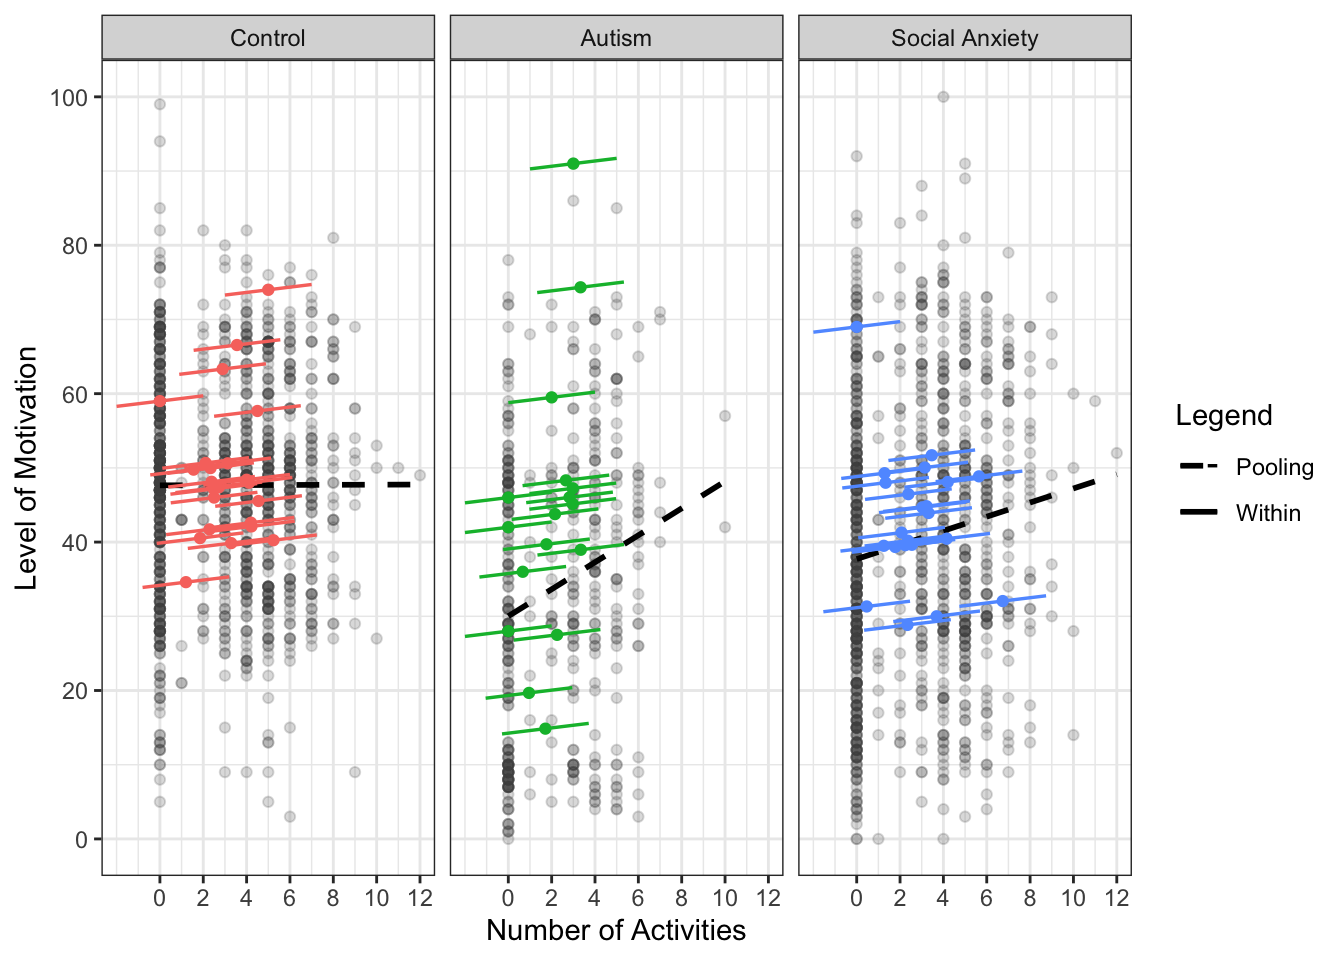
\includegraphics{04_results_files/figure-pdf/fig-groupFE-1.pdf}

}

\caption{\label{fig-groupFE}FE model for motivation vs.~number of
activities by group.}

\end{figure}%

Since the FE models require both an evening survey response for
motivation and the number of activities determined by the DBSCAN-TE
algorithm, some data were lost. This reduced the sample size from 31 to
23 in the control group, from 29 to 17 in the autism group, and from 28
to 22 in the social anxiety group. The FE models need enough data points
for each participant to ensure effective analysis, which explains the
reduction in participants.

\subsubsection{Fixed Effects Models for Motivation and Number of
Activities}\label{fixed-effects-models-for-motivation-and-number-of-activities}

After visualizing the relationships, we proceeded and constructed FE
models separately for each group to better understand how motivation
levels relate to the number of activities engaged in for distinct groups
of individuals. The results from these models are presented in
Table~\ref{tbl-groupFEAnaly}.

\begin{table}

\caption{\label{tbl-groupFEAnaly}FE Models: Motivation and Number of
Activities by Group}

\centering{

\centering
\begin{tabular}[t]{lccc}
\toprule
  & Group: Control & Group: Autism & Group: Social Anxiety\\
\midrule
No. of Activities & 0.259+ & 0.361 & 0.483*\\
 & (1.716) & (1.147) & (2.149)\\
\midrule
No. of Obs. & 1,167 & 451 & 1,033\\
AIC & 9,177.454 & 3,597.049 & 8,797.231\\
R² & 0.003 & 0.003 & 0.004\\
\bottomrule
\multicolumn{4}{l}{\rule{0pt}{1em}Robust t-statistics in parentheses. + p $<$ 0.1, * p $<$ 0.05, ** p $<$ 0.01, *** p $<$ 0.001}\\
\end{tabular}

}

\end{table}%

The results revealed varying relationships across the control, autism,
and social anxiety groups. In the control group, the coefficient was
0.259, suggesting a weakly positive but not strongly significant
association between the number of activities and motivation. For the
autism group, the coefficient was 0.361, also positive but not
significant, indicating that increased activity may have limited direct
impact on motivation in this group. In contrast, the social anxiety
group exhibited a coefficient of 0.483, which was statistically
significant. This suggests a meaningful positive relationship: as
activity levels increase, motivation also increases among individuals
with social anxiety.

These findings emphasize the value of modeling by group and accounting
for individual differences. While engaging in more activities appears to
significantly benefit motivation levels for those with social anxiety,
similar effects were not observed in the control or autism groups. This
may indicate that other factors might play a more critical role in
influencing motivation levels for the control and autism group.

\subsection{Activity Types}\label{activity-types}

To deepen our understanding of how activity engagement influences
motivation, we next explored whether the \emph{type} of location visited
played a role. Specifically, we examined how the number of activities at
certain location categories---such as parks, grocery stores, and
libraries---impacted motivation levels. The analysis incorporated
activity counts derived from the DBSCAN-TE algorithm, as well as
seven-day and 14-day moving averages to capture short- and medium-term
behavioral trends.

While all location types and time windows were considered, only a few
yielded statistically significant results. These findings highlight the
importance of considering both the quantity and context of activities
when analyzing travel behavior and mental well-being.

\subsubsection{Activities at Parks and Grocery
Stores}\label{activities-at-parks-and-grocery-stores}

Building on the general relationship between activity levels and
motivation, we further investigated how specific types of activities at
different locations influence motivation within each group.

When examining park-related activities, statistically significant
results were found exclusively for the control group.
Table~\ref{tbl-groupFEParks} presents the FE models for the seven-day
rolling average number of activities at parks for the three groups.
Specifically, each additional park activity within a seven-day period
was associated with a 3.017-point increase in motivation level. This
suggests that more frequent park visits are linked to heightened
motivation among individuals without a psychiatric diagnosis. However,
no significant relationship was observed between park visits and
motivation for individuals in the autism or social anxiety groups,
indicating that park activities during the observed time frame may not
meaningfully influence motivation for these populations.

\begin{table}

\caption{\label{tbl-groupFEParks}FE Models: Motivation and Number of
Activities at Parks by Group}

\centering{

\centering
\begin{tabular}[t]{lccc}
\toprule
  & Group: Control & Group: Autism & Group: Social Anxiety\\
\midrule
Seven-Day Park & 3.017* & 4.938 & 1.511\\
 & (2.239) & (0.857) & (0.207)\\
\midrule
No. of Obs. & 1,840 & 774 & 1,597\\
AIC & 14,509.34 & 6,215.856 & 13,615.11\\
R² & 0.002 & 0.001 & 0\\
\bottomrule
\multicolumn{4}{l}{\rule{0pt}{1em}Robust t-statistics in parentheses. + p $<$ 0.1, * p $<$ 0.05, ** p $<$ 0.01, *** p $<$ 0.001}\\
\end{tabular}

}

\end{table}%

In contrast, grocery store visits revealed more complex patterns across
the groups. Table~\ref{tbl-groupFEGrocery} presents the FE models for
the number of activities at grocery stores for the three groups. For the
autism group, a statistically significant negative correlation emerged:
each additional grocery store activity was associated with a 2.725-point
decrease in motivation. A similar, though less significant, effect was
found for the control group, with each additional daily grocery store
activity linked to a 2.690-point drop in motivation. The social anxiety
group, however, did not show any statistically significant associations.
These results suggest that grocery store visits, particularly for
autistic individuals, may be associated with increased stress or lower
well-being, thus reducing motivation.

\begin{table}

\caption{\label{tbl-groupFEGrocery}FE Models: Motivation and Number of
Activities at Grocery Stores by Group}

\centering{

\centering
\begin{tabular}[t]{lccc}
\toprule
  & Group: Control & Group: Autism & Group: Social Anxiety\\
\midrule
Grocery Store & -2.690+ & -2.725*** & 0.519\\
 & (-1.878) & (-3.721) & (0.614)\\
\midrule
No. of Obs. & 1,167 & 451 & 1,033\\
AIC & 9,178.666 & 3,598.227 & 8,801.453\\
R² & 0.002 & 0.001 & 0\\
\bottomrule
\multicolumn{4}{l}{\rule{0pt}{1em}Robust t-statistics in parentheses. + p $<$ 0.1, * p $<$ 0.05, ** p $<$ 0.01, *** p $<$ 0.001}\\
\end{tabular}

}

\end{table}%

\subsubsection{Activity Impact on
Motivation}\label{activity-impact-on-motivation}

These findings highlight the importance of considering not only how much
individuals engage in activities, but also where those activities take
place. The varying effects of activity location on motivation across
groups underscore the need for location-specific and group-sensitive
strategies when evaluating the impact of travel behavior on mental
well-being. For the control group, the positive correlation between park
visits and motivation suggests that outdoor environments may play a
beneficial role in supporting overall well-being. In contrast, the
negative relationship between grocery store visits and motivation in the
autism group points to the potential stress associated with routine,
often overstimulating environments.

These group-specific patterns are important because they reveal how
everyday activities can influence mental well-being differently
depending on individual needs and diagnoses. For example, promoting park
visits may be particularly effective in enhancing well-being among the
general population, while interventions aimed at reducing sensory stress
in grocery store environments could support better outcomes for autistic
individuals. Notably, for individuals with social anxiety, the strong
positive relationship between activity levels and motivation suggests
that simply encouraging more engagement in daily activities, regardless
of location, may be especially beneficial. While specific settings may
not significantly impact motivation in this group, the act of
participating in activities itself appears to support mental well-being.
Together, these findings highlight the importance of tailoring mental
health interventions to both the type of activity and the specific needs
of different groups.

\bookmarksetup{startatroot}

\section{Limitations and Future
Recommendations}\label{limitations-and-future-recommendations}

This study has several important limitations that affect the accuracy
and completeness of the data. First, the quality and consistency of data
collection varied across participants. Since participants were enrolled
for different lengths of time and their phones were not always on or
properly recording, some of the LBS data was sparse or missing. As a
result, a some data had to be excluded, and the DBSCAN-TE algorithm may
not have consistently or accurately identified all activities. Although
we used methods like rolling averages and imputation to address gaps,
decreasing the inconsistencies in data collection could improve the
precision of our findings.

Second, while we could identify \emph{where} participants went, we
lacked data on \emph{how long} they spent at each location. For example,
a visit to a park was recorded, but we couldn't tell whether the
participant stayed for several hours or just passed through. This limits
our ability to assess the relationship between time spent in certain
environments and mental well-being. Because the algorithm detects
activities based on stationary data, short or passive visits may not
reflect meaningful engagement with a location.

Finally, the DBSCAN-TE algorithm, while useful, cannot fully confirm the
exact nature of participants' activities. It's possible that some
activities were misclassified or missed altogether. Without direct input
from participants, such as activity diaries, we cannot be certain which
specific activities took place.

To address these limitations, future studies should focus on improving
data quality and collection consistency, perhaps by encouraging regular
phone use and ensuring the tracking app functions reliably. Capturing
the duration of time spent at activity locations and supplementing LBS
data with participant-reported activity diaries could also improve the
accuracy and depth of analysis. These additions would help researchers
gain a more comprehensive understanding of how different types of
activities, and the time spent doing them, relate to mental well-being.

\bookmarksetup{startatroot}

\section{Conclusions}\label{sec-conclude}

This research explored the critical link between travel behavior and
mental health, focusing on young adults with suicidal ideation. By
analyzing daily activities and movement patterns, we identified
significant differences in activity engagement and motivation levels
across three groups: autistic individuals, individuals with social
anxiety, and a control group. The findings underscore the distinct
challenges faced by each group and the importance of considering these
factors in mental health interventions.

We found that individuals in the control group participated in more
activities and reported higher motivation on average, while autistic
individuals and those with social anxiety engaged in fewer activities
and had lower motivation levels. We also found that the relationship
between activity participation and motivation is not uniform across
groups. A small positive relationship existed between the total number
of activities and motivation levels overall. However, only individuals
with social anxiety showed a statistically significant increase in
motivation with more activity engagement. This suggests that increasing
the number of activities may be particularly beneficial for enhancing
well-being in individuals with social anxiety.

Activity location also played a critical role in shaping motivation.
Park visits over a seven-day period were associated with a significant
increase in motivation for the control group, suggesting that outdoor
green spaces may promote mental well-being in the general population.
Conversely, for autistic individuals, grocery store visits were
significantly linked to decreased motivation, indicating that these
environments may be sources of stress or discomfort. These
location-specific trends highlight the importance of not just how much
individuals participate in activities, but where these activities take
place.

The practical implications of these findings are profound. Understanding
how travel behavior influences motivation and mental health can guide
mental health practitioners in developing targeted strategies. For
example, interventions could focus on mitigating the stressors of
grocery store environments for autistic individuals or promoting greater
activity engagement for individuals with social anxiety to enhance their
well-being.

Overall, this research bridges the gap between travel behavior and
mental health, highlighting the importance of personalized approaches to
mental health care. By considering travel behavior as a key factor in
promoting well-being, we provide a roadmap for future research that can
further explore this intersection, ultimately aiming to enhance the
quality of life for individuals by informing more personalized and
effective mental health strategies.

\bookmarksetup{startatroot}

\section*{Acknowledgments}\label{acknowledgments}
\addcontentsline{toc}{section}{Acknowledgments}

\markboth{Acknowledgments}{Acknowledgments}

This data used in this research was collected with help from an
Interdisciplinary Research Grant at Brigham Young University, and
administered under IRB protocol F2020-242. The investigators on the
overarching grant include Terisa Gabrielsen, Jared Nielsen, and Mikle
South.

\bookmarksetup{startatroot}

\section*{References}\label{references}
\addcontentsline{toc}{section}{References}

\markboth{References}{References}

\phantomsection\label{refs}
\begin{CSLReferences}{1}{0}
\bibitem[\citeproctext]{ref-aylottExploratoryStudyGrocery1998}
Aylott, R., \& Mitchell, V.-W. (1998). An exploratory study of grocery
shopping stressors. \emph{International Journal of Retail \&
Distribution Management}, \emph{26}(9), 362--373.
\url{https://doi.org/10.1108/09590559810237908}

\bibitem[\citeproctext]{ref-baileyRelationshipSocialExperience2020}
Bailey, K. M., Frost, K. M., Casagrande, K., \& Ingersoll, B. (2020).
The relationship between social experience and subjective well-being in
autistic college students: {A} mixed methods study. \emph{Autism},
\emph{24}(5), 1081--1092. \url{https://doi.org/10.1177/1362361319892457}

\bibitem[\citeproctext]{ref-barryAddressingDeterminantsPositive2009}
Barry, M. M. (2009). Addressing the determinants of positive mental
health: {Concepts}, evidence and practice. \emph{International Journal
of Mental Health Promotion}, \emph{11}(3), 4--17.
\url{https://doi.org/10.1080/14623730.2009.9721788}

\bibitem[\citeproctext]{ref-brewsterPublicLibraryTherapeutic2014}
Brewster, L. (2014). The public library as therapeutic landscape: {A}
qualitative case study. \emph{Health \& Place}, \emph{26}, 94--99.
\url{https://doi.org/10.1016/j.healthplace.2013.12.015}

\bibitem[\citeproctext]{ref-dekaTravelPatternsNeeds2016}
Deka, D., Feeley, C., \& Lubin, A. (2016). Travel patterns, needs, and
barriers of adults with autism spectrum disorder: {Report} from a
survey. \emph{Transportation Research Record}, \emph{2542}(1), 9--16.
\url{https://doi.org/10.3141/2542-02}

\bibitem[\citeproctext]{ref-delboscExploringRelativeInfluences2011}
Delbosc, A., \& Currie, G. (2011). Exploring the relative influences of
transport disadvantage and social exclusion on well-being.
\emph{Transport Policy}, \emph{18}(4), 555--562.
\url{https://doi.org/10.1016/j.tranpol.2011.01.011}

\bibitem[\citeproctext]{ref-eliaPublicLibrariesSupporting2019}
Elia, H. (2019). Public libraries supporting health and wellness: {A}
literature review. \emph{School of Information Student Research
Journal}, \emph{9}(2). \url{https://doi.org/10.31979/2575-2499.090207}

\bibitem[\citeproctext]{ref-frimanHowDoesTravel2017}
Friman, M., Gärling, T., Ettema, D., \& Olsson, L. E. (2017). How does
travel affect emotional well-being and life satisfaction?
\emph{Transportation Research Part A: Policy and Practice}, \emph{106},
170--180. \url{https://doi.org/10.1016/j.tra.2017.09.024}

\bibitem[\citeproctext]{ref-hoisingtonTenQuestionsConcerning2019}
Hoisington, A. J., Stearns-Yoder, K. A., Schuldt, S. J., Beemer, C. J.,
Maestre, J. P., Kinney, K. A., Postolache, T. T., Lowry, C. A., \&
Brenner, L. A. (2019). Ten questions concerning the built environment
and mental health. \emph{Building and Environment}, \emph{155}, 58--69.
\url{https://doi.org/10.1016/j.buildenv.2019.03.036}

\bibitem[\citeproctext]{ref-kennyWhichTermsShould2016}
Kenny, L., Hattersley, C., Molins, B., Buckley, C., Povey, C., \&
Pellicano, E. (2016). Which terms should be used to describe autism?
{Perspectives} from the {UK} autism community. \emph{Autism},
\emph{20}(4), 442--462. \url{https://doi.org/10.1177/1362361315588200}

\bibitem[\citeproctext]{ref-kuykendallLeisureEngagementSubjective2015}
Kuykendall, L., Tay, L., \& Ng, V. (2015). Leisure engagement and
subjective well-being: {A} meta-analysis. \emph{Psychological Bulletin},
\emph{141}(2), 364--403. \url{https://doi.org/10.1037/a0038508}

\bibitem[\citeproctext]{ref-lanDailySpacetimeActivities2022}
Lan, Y., Roberts, H., Kwan, M.-P., \& Helbich, M. (2022). Daily
space-time activities, multiple environmental exposures, and anxiety
symptoms: {A} cross-sectional mobile phone-based sensing study.
\emph{Science of The Total Environment}, \emph{834}, 155276.
\url{https://doi.org/10.1016/j.scitotenv.2022.155276}

\bibitem[\citeproctext]{ref-leichsenringSocialAnxietyDisorder2017}
Leichsenring, F., \& Leweke, F. (2017). Social anxiety disorder.
\emph{New England Journal of Medicine}, \emph{376}(23), 2255--2264.
\url{https://doi.org/10.1056/NEJMcp1614701}

\bibitem[\citeproctext]{ref-loadesRapidSystematicReview2020}
Loades, M. E., Chatburn, E., Higson-Sweeney, N., Reynolds, S., Shafran,
R., Brigden, A., Linney, C., McManus, M. N., Borwick, C., \& Crawley, E.
(2020). Rapid systematic review: {The} impact of social isolation and
loneliness on the mental health of children and adolescents in the
context of {COVID-19}. \emph{Journal of the American Academy of Child \&
Adolescent Psychiatry}, \emph{59}(11), 1218--1239.e3.
\url{https://doi.org/10.1016/j.jaac.2020.05.009}

\bibitem[\citeproctext]{ref-lubinTransportationIssuesAdults2016}
Lubin, A., \& Feeley, C. (2016). Transportation issues of adults on the
autism spectrum: {Findings} from focus group discussions.
\emph{Transportation Research Record}, \emph{2542}(1), 1--8.
\url{https://doi.org/10.3141/2542-01}

\bibitem[\citeproctext]{ref-macfarlaneClassifyingLocationPoints2024}
Macfarlane, G. S., Riches, G., Youngs, E. K., \& Nielsen, J. A. (2024).
Classifying location points as daily activities using simultaneously
optimized {DBSCAN-TE} parameters. \emph{Findings}.
\url{https://doi.org/10.32866/001c.116197}

\bibitem[\citeproctext]{ref-mackettMentalHealthTravel2021}
Mackett, R. L. (2021). Mental health and travel behaviour. \emph{Journal
of Transport \& Health}, \emph{22}, 101143.
\url{https://doi.org/10.1016/j.jth.2021.101143}

\bibitem[\citeproctext]{ref-nilssonEffectsTimePressure2017}
Nilsson, E., Gärling, T., \& Marell, A. (2017). Effects of time
pressure, type of shopping, and store attributes on consumers'
satisfaction with grocery shopping. \emph{The International Review of
Retail, Distribution and Consumer Research}, \emph{27}(4), 334--351.
\url{https://doi.org/10.1080/09593969.2017.1309674}

\bibitem[\citeproctext]{ref-orbenEffectsSocialDeprivation2020}
Orben, A., Tomova, L., \& Blakemore, S.-J. (2020). The effects of social
deprivation on adolescent development and mental health. \emph{The
Lancet Child \& Adolescent Health}, \emph{4}(8), 634--640.
\url{https://doi.org/10.1016/S2352-4642(20)30186-3}

\bibitem[\citeproctext]{ref-ozturkRelationshipAttachmentStyle2010}
Öztürk, A., \& Mutlu, T. (2010). The relationship between attachment
style, subjective well-being, happiness and social anxiety among
university students'. \emph{Procedia - Social and Behavioral Sciences},
\emph{9}, 1772--1776. \url{https://doi.org/10.1016/j.sbspro.2010.12.398}

\bibitem[\citeproctext]{ref-pelgrimsAssociationUrbanEnvironment2021}
Pelgrims, I., Devleesschauwer, B., Guyot, M., Keune, H., Nawrot, T. S.,
Remmen, R., Saenen, N. D., Trabelsi, S., Thomas, I., Aerts, R., \& De
Clercq, E. M. (2021). Association between urban environment and mental
health in {Brussels}, {Belgium}. \emph{BMC Public Health}, \emph{21}(1),
635. \url{https://doi.org/10.1186/s12889-021-10557-7}

\bibitem[\citeproctext]{ref-pousoContactBluegreenSpaces2021}
Pouso, S., Borja, Á., Fleming, L. E., Gómez-Baggethun, E., White, M. P.,
\& Uyarra, M. C. (2021). Contact with blue-green spaces during the
{COVID-19} pandemic lockdown beneficial for mental health. \emph{Science
of The Total Environment}, \emph{756}, 143984.
\url{https://doi.org/10.1016/j.scitotenv.2020.143984}

\bibitem[\citeproctext]{ref-rateringMovingAnxietyDisorder2024}
Ratering, C., van der Heijden, R., \& Martens, K. (2024). Moving around
with an anxiety disorder. \emph{Transportation Research Part F: Traffic
Psychology and Behaviour}, \emph{100}, 493--506.
\url{https://doi.org/10.1016/j.trf.2023.12.005}

\bibitem[\citeproctext]{ref-rautioLivingEnvironmentIts2018}
Rautio, N., Filatova, S., Lehtiniemi, H., \& Miettunen, J. (2018).
Living environment and its relationship to depressive mood: {A}
systematic review. \emph{International Journal of Social Psychiatry},
\emph{64}(1), 92--103. \url{https://doi.org/10.1177/0020764017744582}

\bibitem[\citeproctext]{ref-richesTransformingGPSPoints2022}
Riches, G. (2022). \emph{Transforming {GPS} points to daily activities
using simultaneously optimized {DBSCAN-TE} parameters} {[}PhD thesis{]}.
Brigham Young University.

\bibitem[\citeproctext]{ref-ridgwaySubjectiveWellbeingAutistic}
Ridgway, K., Macmillan, C., Demmer, D. H., Hooley, M., Hedley, D.,
Westrupp, E., \& Stokes, M. A. (2024). Subjective wellbeing of autistic
adolescents and young adults: {A} cross sectional study. \emph{Autism
Research}, \emph{n/a}(n/a). \url{https://doi.org/10.1002/aur.3139}

\bibitem[\citeproctext]{ref-stanleyMobilitySocialExclusion2011}
Stanley, J. K., Hensher, D. A., Stanley, J. R., \& Vella-Brodrick, D.
(2011). Mobility, social exclusion and well-being: {Exploring} the
links. \emph{Transportation Research Part A: Policy and Practice},
\emph{45}(8), 789--801. \url{https://doi.org/10.1016/j.tra.2011.06.007}

\bibitem[\citeproctext]{ref-syahputriEffectTravelSatisfaction2022}
Syahputri, J., Dharmowijoyo, D. B. E., Basuki Joewono, T., \& Rizki, M.
(2022). Effect of travel satisfaction and heterogeneity of
activity-travel patterns of other persons in the household on social and
mental health: {The} case of {Bandung Metropolitan} area. \emph{Case
Studies on Transport Policy}, \emph{10}(4), 2111--2124.
\url{https://doi.org/10.1016/j.cstp.2022.09.005}

\bibitem[\citeproctext]{ref-takiguchiRelationshipLeisureActivities2022}
Takiguchi, Y., Matsui, M., Kikutani, M., \& Ebina, K. (2022). The
relationship between leisure activities and mental health: {The} impact
of resilience and {COVID}-19. \emph{Applied Psychology. Health and
Well-Being}, 10.1111/aphw.12394.
\url{https://doi.org/10.1111/aphw.12394}

\bibitem[\citeproctext]{ref-whiteAssociationsGreenBlue2021}
White, M. P., Elliott, L. R., Grellier, J., Economou, T., Bell, S.,
Bratman, G. N., Cirach, M., Gascon, M., Lima, M. L., Lõhmus, M.,
Nieuwenhuijsen, M., Ojala, A., Roiko, A., Schultz, P. W., van den Bosch,
M., \& Fleming, L. E. (2021). Associations between green/blue spaces and
mental health across 18 countries. \emph{Scientific Reports},
\emph{11}(1), 8903. \url{https://doi.org/10.1038/s41598-021-87675-0}

\bibitem[\citeproctext]{ref-wooldridgeIntroductoryEconometricsModern2009}
Wooldridge, J. (2009). \emph{Introductory {Econometrics}: {A Modern
Appraoch}} (4th ed.). South-Western Cengage Learning.

\bibitem[\citeproctext]{ref-yanosNegativeSupportiveSocial2001}
Yanos, P. T., Rosenfield, S., \& Horwitz, A. V. (2001). Negative and
supportive social interactions and quality of life among persons
diagnosed with severe mental illness. \emph{Community Mental Health
Journal}, \emph{37}(5), 405--419.
\url{https://doi.org/10.1023/A:1017528029127}

\bibitem[\citeproctext]{ref-yeSocialAnxietySubjective2021}
Ye, B., Li, L., Wang, P., Wang, R., Liu, M., Wang, X., \& Yang, Q.
(2021). Social anxiety and subjective well-being among {Chinese} college
students: {A} moderated mediation model. \emph{Personality and
Individual Differences}, \emph{175}, 110680.
\url{https://doi.org/10.1016/j.paid.2021.110680}

\end{CSLReferences}



\end{document}
